\documentclass[final,hyperref={pdfpagelabels=false}]{beamer}
\usepackage{grffile}
\mode<presentation>{\usetheme{PosterLogProb}}
%\mode<presentation>{\usetheme{I6pd2}}
\usepackage[english]{babel}
\usepackage[latin1]{inputenc}
\usepackage{amsmath,amsthm, amssymb, latexsym}
\usepackage{epsfig}

%\usepackage{algorithm}
%\usepackage{algorithmic}

%\usepackage{times}\usefonttheme{professionalfonts}  % obsolete
%\usefonttheme[onlymath]{serif}
%\boldmath
\usepackage[orientation=portrait,size=a0,scale=1.4,debug]{beamerposter}
% change list indention level
% \setdefaultleftmargin{3em}{}{}{}{}{}
\providecommand\thispdfpagelabel[1]{}
\setbeamertemplate{bibliography entry title}{\color{black}}
\setbeamertemplate{bibliography entry location}{}
\setbeamertemplate{bibliography entry note}{}


%\usepackage{snapshot} % will write a .dep file with all dependencies, allows for easy bundling

\usepackage{array,booktabs,tabularx}
\newcolumntype{Z}{>{\centering\arraybackslash}X} % centered tabularx columns
\newcommand{\pphantom}{\textcolor{ta3aluminium}} % phantom introduces a vertical space in p formatted table columns??!!

\listfiles

\usepackage{amsthm}
%%%%%%%%%%%%%%%%%%%%%%%%%%%%%%%%%%%%%%%%%%%%%%%%%%%%%%%%%%%%%%%%%%%%%%%%%%%%%%%%%%%%%%


 \title{\huge\bfseries\hspace*{-1em} Mezuro: Understanding source code metrics}
\date{}
\author{\large Dylan Guedes
\and Diego Camarinha
\and Rafael Manzo
\and Paulo Meirelles
}

\institute{Faculty Gama (FGA) -- University of Bras�lia (UnB), Brazil
  \and
  Institute of Mathematics and Statistics -- University of S�o Paulo (USP), Brazil
  }

%%%%%%%%%%%%%%%%%%%%%%%%%%%%%%%%%%%%%%%%%%%%%%%%%%%%%%%%%%%%%%%%%%%%%%%%%%%%%%%%%%%%%%
\newlength{\columnheight}
\setlength{\columnheight}{105cm}


%%%%%%%%%%%%%%%%%%%%%%%%%%%%%%%%%%%%%%%%%%%%%%%%%%%%%%%%%%%%%%%%%%%%%%%%%%%%%%%%%%%%%%
\begin{document}
\begin{frame}
  \begin{columns}
    % ---------------------------------------------------------%
    % Set up a column 
    \begin{column}{.49\textwidth}
      \begin{beamercolorbox}[center,wd=\textwidth]{postercolumn}
        \begin{minipage}[T]{.95\textwidth}  % tweaks the width, makes a new \textwidth
          \parbox[t][\columnheight]{\textwidth}{ % must be some better way to set the the height, width and textwidth simultaneously
            % Since all columns are the same length, it is all nice and tidy.  You have to get the height empirically
            % ---------------------------------------------------------%
            % fill each column with content
%\vfill
\begin{block}{What is Mezuro}
  \begin{itemize}

	\item Mezuro is a FOSS web-based platform that analyzes source code.

    \item It allows developers to compare analyzed projects and share knowledge
        about metrics.

    \item Mezuro main goal is to help software developers and maintainers to understand
        and feel comfortable to use source code metrics during their projects.
        
  \end{itemize}              
\end{block}

%-------------------------------------------------------------------------------
\vfill
\begin{block}{Why Mezuro?}
	\begin{itemize}
        \item 100\% FOSS solution;

        \item Continuously generate reviews about a project, via customized
            scheduling;

        \item It allows a level of metrics configuration and composition that
            is not available in other tools analyzed.

	\end{itemize}
\end{block}


%-------------------------------------------------------------------------------
\vfill
\begin{block}{Mezuro features}
	\begin{itemize}

        \item Mezuro features related to a project, responsible for defining
            Mezuro as a source code metrics platform:
            \begin{itemize}
                \item Obtain and evaluate source code from compressed file or
                    tools such as Git, Subversion, and Bazaar;
                \item Code processing scheduling;
                \item Use of multiple metrics configurations for multiple
                    projects;
                \item Visualization of results per file via plot graphics;
                \item Extensible architecture to include new metric collectors;
                \item Public results that are accessible by the community.
            \end{itemize}

        \item Mezuro features related to metric configurations, responsible
            for allowing definitions and spread of metrics configurations, being
            one of its stand out factors among the others platforms:
            \begin{itemize}
                \item Metrics creation;
                \item Metrics configuration cloning, giving users a quick start
                    to rate their projects, and the option to use already well
                    established metrics configuration;
                \item Statistics about most popular configurations in the
                    community;
                \item Creation of ``reading groups'' to be used in textual
                    interpretation of metrics results;
                \item Configuration of qualitative ranges associated with
                    value of metrics;
                \item Combination of native metrics to create composed and more
                    complex analysis.
            \end{itemize}

	\begin{figure}
	  \begin{center}
	    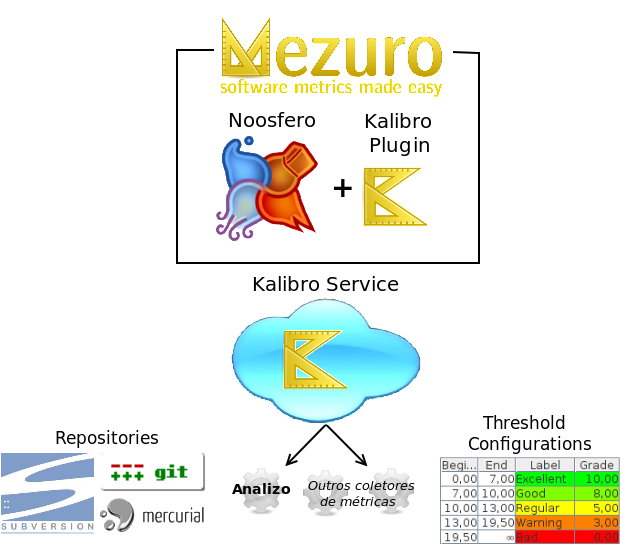
\includegraphics[scale=1.5]{figures/interactions.png}
	    \caption{kalibro interation diagram.}
	    \label{fig:background:free-software-repository}
	  \end{center}
	\end{figure}

	\end{itemize}
\end{block}

\vfill
        

}
\end{minipage}
\end{beamercolorbox}
\end{column}
% ---------------------------------------------------------%
% end the column

% ---------------------------------------------------------%
% Set up a column 
\begin{column}{.49\textwidth}
  \begin{beamercolorbox}[center,wd=\textwidth]{postercolumn}
    \begin{minipage}[T]{.95\textwidth} % tweaks the width, makes a new \textwidth
      \parbox[t][\columnheight]{\textwidth}{ % must be some better way to set the the height, width and textwidth simultaneously
        % Since all columns are the same length, it is all nice and tidy.  You have to get the height empirically
        % ---------------------------------------------------------%
        % fill each column with content

        \begin{block}{Mezuro Architecture}

	\begin{itemize}
        \item Mezuro is composed of three parts: the configuration prior to
            the analysis; (ii) source code metrics computation and evaluation;
            (iii) and a graphic interface to present results.

        \item Currently, both the computation and visualization modules use
            other tools developed in the Mezuro project: \textbf{Kalibro} and
            \textbf{Prezento}.

        \item Mezuro architecture evolved to a microservice architecture, to:
            minimize the amount of code to maintain; test and grant quality of
            code; and modularize the application in several independent services.

        \item \textbf{Kalibro} is the base of the architecture, and its
            segmented in three smaller entities:

            \begin{itemize}
                \item \textbf{Kalibro Processor}, responsible for processing and
                    evaluating metrics;
                \item \textbf{Kalibro Configurations}, responsible for metrics
                    definitions and configurations;
                \item \textbf{Kalibro Client}, responsible for interoperate
                    communications between these entities.
            \end{itemize}

        \item \textbf{Prezento}, the presentation layer, mainly communicates with
            Kalibro Processor and Kalibro Configurations, via the Kalibro
            Client interface.

        \end{itemize}
          	
        \end{block}
             
\vfill
      }
      % ---------------------------------------------------------%
      % end the column
        \end{minipage}
      \end{beamercolorbox}
    \end{column}
    % ---------------------------------------------------------%
    % end the column
  \end{columns}
  %\vskip1ex
  % \tiny\hfill\textcolor{ta2gray}{Created with \LaTeX \texttt{beamerposter}  \url{http://www-i6.informatik.rwth-aachen.de/~dreuw/latexbeamerposter.php}}
  
\end{frame}
\end{document}


%%%%%%%%%%%%%%%%%%%%%%%%%%%%%%%%%%%%%%%%%%%%%%%%%%%%%%%%%%%%%%%%%%%%%%%%%%%%%%%%%%%%%%%%%%%%%%%%%%%%
%%% Local Variables: 
%%% mode: latex
%%% TeX-PDF-mode: t
%%% End:

% LocalWords:  ABox ABoxes PSAT
